\documentclass[a4paper, 11pt]{article}
\usepackage{hyperref}
\usepackage[margin=0.5in]{geometry}

\usepackage[version=3]{mhchem}
\usepackage[arrowdel]{physics}
\usepackage{siunitx}

\newcommand{\au}{\text{a.u.}}
\newcommand{\kb}{\ensuremath{k_{\text{b}}}}
\newcommand{\din}[2][]{\text{đ}^{#1}#2}
\newcommand{\del}[3][]{\partial_{#2}^{#1}#3}
\newcommand{\fix}[2]{\left(#1\right)_{#2}}
\newcommand{\integ}[5][]{\int\limits_{#2}^{#3}\dd[#1]{#4}#5}
\newcommand{\intin}[5][]{\int\limits_{#2}^{#3}\din[#1]{#4}#5}

\title{Summary of SI1162 Statistical Physics}
\author{Yashar Honarmandi \\ yasharh@kth.se}
\date{\today}

\begin{document}

\maketitle

\begin{abstract}
	Detta ær en sammanfattning av kursen SH1014 Modern fysik.
\end{abstract}

\pagenumbering{roman}
\thispagestyle{empty}

\newpage

\tableofcontents

\newpage

\pagenumbering{arabic}

\section{Useful Mathematics}

\paragraph{A Useful Commutation Relation}
You might happen upon commutation relations of the form $\comm{f(A)}{B}$ show up. We would like to try to simplify it for the particular case where $\comm{A}{B} = C$, where $C$ is some operator commuting with $A$. To do this, we first study $\comm{A^{n}}{B}$ in a general case. We have
\begin{align*}
	\comm{A^{n}}{B} = A\comm{A^{n - 1}}{B} + \comm{A}{B}A^{n - 1},
\end{align*}
prompting us to find this commutator by induction. For $n = 2$ we have
\begin{align*}
	\comm{A^{2}}{B} = A\comm{A}{B} + \comm{A}{B}A.
\end{align*}
For $n = 3$ we obtain
\begin{align*}
	\comm{A^{3}}{B} = A\comm{A^{2}}{B} + \comm{A}{B}A^{2} = A(A\comm{A}{B} + \comm{A}{B}A) + \comm{A}{B}A^{2} = A^{2}\comm{A}{B} + A\comm{A}{B}A + \comm{A}{B}A^{2}.
\end{align*}
A suitable induction hypothesis looks to be
\begin{align*}
	\comm{A^{n}}{B} = \sum\limits_{k = 1}^{n}A^{n - k}\comm{A}{B}A^{k - 1}.
\end{align*}
Assuming it to be true, we have
\begin{align*}
	\comm{A^{n + 1}}{B} &= A\comm{A^{n}}{B} + \comm{A}{B}A^{n} \\
	                    &= A\sum\limits_{k = 1}^{n}A^{n - k}\comm{A}{B}A^{k - 1} + \comm{A}{B}A^{n} \\
	                    &= \sum\limits_{k = 1}^{n}A^{n + 1 - k}\comm{A}{B}A^{k - 1} + \comm{A}{B}A^{n} \\
	                    &= \sum\limits_{k = 1}^{n + 1}A^{n + 1 - k}\comm{A}{B}A^{k - 1},
\end{align*}
proving the hypothesis by induction.

Now we write
\begin{align*}
	f(A) = \sum\limits_{n = 0}^{\infty}\frac{1}{n!}f_{n}A^{n}
\end{align*}
to obtain
\begin{align*}
	\comm{f(A)}{B} &= \comm{\sum\limits_{n = 0}^{\infty}\frac{1}{n!}f_{n}A^{n}}{B} \\
	               &= \sum\limits_{n = 0}^{\infty}\frac{1}{n!}f_{n}\comm{A^{n}}{B} \\
	               &= \sum\limits_{n = 0}^{\infty}\frac{1}{n!}f_{n}\sum\limits_{k = 1}^{n}A^{n - k}\comm{A}{B}A^{k - 1}.
\end{align*}
Assuming $\comm{A}{B}$ to commute with $A$, we have
\begin{align*}
	\comm{f(A)}{B} &= \sum\limits_{n = 0}^{\infty}\frac{1}{n!}f_{n}A^{n - 1}\comm{A}{B}\sum\limits_{k = 1}^{n} \\
	               &= \comm{A}{B}\sum\limits_{n = 1}^{\infty}\frac{1}{(n - 1)!}f_{n}A^{n - 1} \\
	               &= \comm{A}{B}\sum\limits_{m = 0}^{\infty}\frac{1}{m!}f_{m + 1}A^{m} \\
	               &= \comm{A}{B}\dv{f}{A}.
\end{align*}

\paragraph{Symmetries on Hilbert Space}
A symmetry on Hilbert space is a transformation that leaves all inner products unaltered.

\paragraph{Wigner's Theorem}
Wigner's theorem states that any operator that is a symmetry is either unitary or anti-unitary (the latter meaning $\mel{\Phi}{\adj{U}U}{\Psi} = \braket{\Psi}{\Phi}$).

\paragraph{Transformation of Operators}
Consider a symmetry operator $u$. In order for this to be a symmetry, it must also act on all operators according to $A\to uA\adj{u}$.

\paragraph{Continuous Symmetries}
Continuous symmetries are found in two forms: One which operates on the coefficients of the state and one which operates on the basis vectors. Denoting some symmetry as $u_{\var{\theta}}$, which changes $\theta$ to $\var{\theta}$, we require symmetries to have the following properties:
\begin{itemize}
	\item $u_{\var{\theta_{1}}}u_{\var{\theta_{2}}} = u_{\var{\theta_{1}} + \var{\theta_{2}}}$.
	\item $u_{\var{\theta}}^{-1} = u_{-\var{\theta}}$.
	\item $\lim\limits_{\var{\theta} \to 0}u_{\var{\theta}} = 1$.
\end{itemize}

\paragraph{Generators of Continuous Symmetries}
Continuous symmetry operators are smooth maps acting on a manifold - namely, Hilbert space. Hence we can use the language of Lie algebra to study them (if you know nothing about Lie algebra, pretend that I didn't write this and carry on. If you want some reference material, please look at my summary of SI2360). We expand the symmetry operator around the identity as
\begin{align*}
	u_{\var{\theta}} = 1 - i\var{\theta}T + \dots
\end{align*}
for some operator $T$. We have
\begin{align*}
	\adj{u_{\var{\theta}}}u_{\var{\theta}} = (1 + i\var{\theta}\adj{T})(1 - i\var{\theta}T) = 1 + i\var{\theta}\left(T - \adj{T}\right) + \dots,
\end{align*}
where we have ignored higher-order terms in $\var{\theta}$. The requirement that the symmetry be unitary yields $\adj{T} - T = 0$, and hence the generator $T$ is self-adjoint. By continuous application of this we obtain
\begin{align*}
	u_{\var{\theta}} = e^{-i\var{\theta}T}.
\end{align*}
This operator satisfies all of the above criteria for a continuous symmetry.

\paragraph{Effect of Symmetries on Wavefunctions}
Let $u_{\var{\theta}}$ act on $\theta$ and $\vb{x}$ be a vector containing any other parameters describing the basis. We have
\begin{align*}
	u_{\var{\theta}}\ket{\Psi} = \integ{}{}{\vb{x}}{\integ{}{}{\theta}{u_{\var{\theta}}\ket{\theta, \vb{x}}\braket{\theta, \vb{x}}{\Psi}}} = \integ{}{}{\vb{x}}{\integ{}{}{\theta}{\ket{\theta + \var{\theta}, \vb{x}}\braket{\theta, \vb{x}}{\Psi}}} = \integ{}{}{\vb{x}}{\integ{}{}{\theta}{\ket{\theta, \vb{x}}\braket{\theta - \var{\theta}, \vb{x}}{\Psi}}},
\end{align*}
meaning that the symmetry transforms $\Psi(\theta, \vb{x})$ to $\Psi(\theta - \var{\theta}, \vb{x})$.

Suppose instead that $\theta$ parametrizes the coefficients - in other words, $\ket{\Psi(\theta)} = \Psi(\theta, \vb{x})\ket{\vb{x}}$. In this case, the symmetry transforms the wavefunction to $\Psi(\theta + \var{\theta}, \vb{x})$.

\paragraph{Commutation Relations Between Parameters and Generators}
For a symmetry of the first kind, we use the transformation rule for operators to obtain commutation relations between parameters and their generators. More specifically, we require
\begin{align*}
	(1 - i\var{\theta}T)\theta(1 + i\var{\theta}T) = \theta + \var{\theta}
\end{align*}
to first order. The left-hand side is given by
\begin{align*}
	\theta + i\var{\theta}\theta T - i\var{\theta}(T\theta + i\var{\theta}T\theta T) = \theta + i\var{\theta}\comm{\theta}{T}
\end{align*}
to first order, implying
\begin{align*}
	i\comm{\theta}{T} = 1.
\end{align*}

\paragraph{Generators in the Operator Basis}
We have
\begin{align*}
	\left(1 - i\var{\theta}T\right)\ket{\Psi} &= \integ{}{}{\vb{x}}{\integ{}{}{\theta}{\ket{\theta, \vb{x}}\mel{\theta, \vb{x}}{\left(1 - i\var{\theta}T\right)}{\Psi}}} \\
	                                          &= \integ{}{}{\vb{x}}{\integ{}{}{\theta}{\ket{\theta, \vb{x}}\braket{\theta - \var{\theta}, \vb{x}}{\Psi}}} \\
	                                          &= \integ{}{}{\vb{x}}{\integ{}{}{\theta}{\ket{\theta, \vb{x}}\left(\braket{\theta, \vb{x}}{\Psi} - \var{\theta}\del{\theta}{\braket{\theta, \vb{x}}{\Psi}}\right)}},
\end{align*}
implying
\begin{align*}
	\bra{\theta, \vb{x}}T = \frac{1}{i}\del{\theta}{}.
\end{align*}

\paragraph{Discrete Symmetries}
A discrete symmetry is an operator for which the previously stated machinery does not hold.

\paragraph{Complex Conjugation}

\paragraph{Tensors}
A tensor of rank $n$ is a multilinear map from $n$ vectors in some vector space to a scalar.

It is clear that the set of tensors of some rank form a vector space, and so we would like to identify some basis for the space of tensors.

\paragraph{Basis for $n = 1$}
We start with rank $1$ tensors. The inner product is certainly a rank $1$ tensor according to the definition, and so we would like to use that. Now let the set of $v_{i}$ denote the set of orthonormal basis vectors for the space $V$. We then choose the basis
\begin{align*}
	e_{i}(v) = \bra{v_{i}}{v}
\end{align*}
as the basis for the set of rank $1$ tensors. This may also be denoted simply as the tensor $v_{i}$ (the confusion will disappear later).

\paragraph{The Tensor Product}
To find a basis for tensors of higher order, we first need to introduce the tensor product. We define it for rank $1$ tensors as
\begin{align*}
	s(v)\otimes t(w) = \braket{s}{v}\braket{t}{w}.
\end{align*}
The tensor product has allowed us to construct a rank $2$ tensor from two rank $1$ tensors. Repeatedly applying it allows us to construct tensors of any rank. The tensor product is also bilinear, in line with our definition.

\paragraph{The Tensor Product of Operators}
It follows naturally that
\begin{align*}
	(S\otimes T)(v\otimes w) = S(v)\otimes T(w).
\end{align*}

\section{Combinatorics}

\paragraph{Combinations and permutations}
Permutations are sequences of some kind. Combinations are permutations where order does not matter. From a collection of $n$ elements, the number of possible permutations of $k$ elements is
\begin{align*}
	\Omega = \frac{n!}{(n - k)!}
\end{align*}
and the number of possible combinations is
\begin{align*}
	\Omega = \binom{n}{k}.
\end{align*}

\section{Grundläggande koncept}

\paragraph{Syftet med reglerteknik}
Reglerteknik handlar om att kontrollera olika storheter, ofta betecknad $y$, i ett system mot något värde, ofta betecknad $r$. I tillägg till systemets egna beteende påverkas storheten vi vill reglera typiskt av en yttre störning $v$. Vi kan reglera systemet genom att tillföra en påverkan, ofta betecknad $u$.

\paragraph{Strategi}
För att förstå systemet, tar vi först fram en modell som beskriver det. Ur denna modellen fås typiskt en differentialekvation. Denna löser vi med Laplacetransform över tid.

\paragraph{Överförningsfungktionen}
För linjära system fås en lösning i Laplacerummet på formen $Y(s) = G(s)U(s)$, där $U$ är Laplacetransformen av $u$. Funktionen $G$ är överförningsfunktionen. Notera att denna lösningsformen typiskt beror på att alla initialvärden är $0$.

\paragraph{Poler}
Ett systems poler är rötterna till nämnarpolynomet (som typiskt finns) i överförningsfunktionen.

\paragraph{Stabilitet}
Ett system är stabilt om det tenderar mot ett visst läge efter lång tid. Systemets stabilitet är typiskt kopplad med dets poler. Detta kan man se i enkla fall, till exempel vanliga linjära ordinära differentialekvationer. Här är systemet stabilt om det inte finns några poler i högre halvplan, och avståndet längs med reella axeln anger hur snabbt lösningen tenderar mot det stabila läget.

\paragraph{Nollställen}
Ett systems nollställen är rötterna till täljarpolynomet (som typiskt finns) hos överförningsfunktioner. Eftersom vi är intresserade av att styra $y$, är det viktigt hur vi ska välja $u$ för att få det. Därmed är $\frac{1}{G}$ en viktig storhet, och nollställen kan därmed orsaka reglerproblem som är svårlösta.

\paragraph{Impulssvar}
Om lösningen för $Y$ är på formen $Y = GU$, är lösningen för $y$ på formen
\begin{align*}
	y(t) = \integ{0}{t}{\tau}{g(\tau)u(t - \tau)}.
\end{align*}
$g$ kallas för impulssvaret.

\paragraph{Blockschema}
Ett blockschema är ett systematisk sätt att rita reglerade system på. För att förstå hur man läser dem, betrakta figur \ref{fig:basic_block}.
\begin{figure}[!ht]
	\centering
	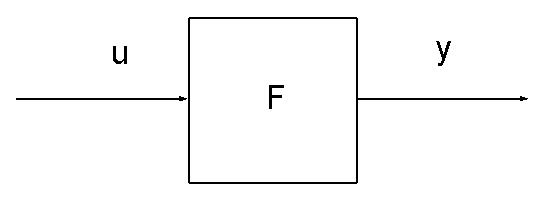
\includegraphics[width = 0.5\textwidth]{./Images/basic_block.eps}
	\caption{Illustration av ett enkelt blockschema.}
	\label{fig:basic_block}
\end{figure}

Med denna figuren menas att $Y(s) = F(s)U(s)$.

\paragraph{Rotort}
En rotort är en plott av ett systems poler som funktion av någon parameter. Den är typiskt uppdelad i grenar, som är kurvor i planet som är parametriserade av parametervärdet. Polerna som motsvarar parametervärdet $0$ är rotortens startpunkter, och polarna motsvarande parametervärdet $\infty$ är rotortens ändpunkter. Om rotorten närmar sig kurvor, är dessa rotortens asymptoter.

\section{Ensembles}

\paragraph{Definition}
For a given system, an ensemble is a collection of all possible states of the system such that a certain set of quantities are preserved.

\paragraph{The Microcanonical Ensemble}
The microcanonical ensemble has $N_{i}$, $V$ and $E$ preserved.

\paragraph{The Canonical Ensemble}
The canonical ensemble has $N_{i}$, $V$ and $T$ preserved.

\paragraph{The Grand Canonical Ensemble}
The grand canonical ensemble has $\mu_{i}$, $V$ and $T$ preserved.

\section{Gases}

\paragraph{The Maxwell-Boltzmann Velocity Distribution}
Consider a system of $n$ (approximately) non-interacting particles. Assuming the separations to be much larger than the particle size and neglecting rotational and vibrational degrees of freedom, each particle has total energy $E = \frac{1}{2}mv^{2}$. We can now treat each particle as a small system in contact with a heat reservoir (namely the other particles). The results concerning the Boltzmann factor thus hold for this molecule. A single velocity component is thus described by the probability distribution
\begin{align*}
	g(v_{i}) = \sqrt{\frac{m}{2\pi\kb T}}e^{-\frac{mv_{i}^{2}}{2\kb T}}.
\end{align*}
This is of course true for all particles in the gas, meaning that the fraction of molecules with $v_{i}$ in the range $v_{i}$ to $v_{i} + \dd{v_{i}}$ is equal to $g(v_{i})\dd{v_{i}}$.

It can be shown that
\begin{align*}
	\expval{v_{i}} = 0,\ \expval{\abs{v_{i}}} = \sqrt{\frac{2\kb T}{m}},\ \expval{v_{i}^{2}} = \frac{\kb T}{m}.
\end{align*}

\paragraph{The Maxwell-Boltzmann Speed Distribution}
Consider instead the distribution of the particle speed. The distribution satisfying that the fraction of particles with speed in the range $v$ to $v + \dd{v}$ is
\begin{align*}
	f(v) = \frac{4}{\sqrt{\pi}}\left(\frac{m}{2\kb T}\right)^{\frac{3}{2}}v^{2}e^{-\frac{v^{2}}{2\kb T}},
\end{align*}
where the quadratic factor arises due to the integration volume.

It can be shown that
\begin{align*}
	\expval{v} = \sqrt{\frac{8\kb T}{\pi m}},\ \expval{v^{2}} = \frac{3\kb T}{m}
\end{align*}
and that $f$ has a maximum for
\begin{align*}
	v = \sqrt{\frac{2\kb T}{m}}.
\end{align*}

\paragraph{Directions and the Speed Distribution}
Because the velocity distribution is isotropic, the fraction of molecules whose trajectories lie in some solid angle range $\dd{\Omega}$ is given by $\frac{\dd{\Omega}}{4\pi}$. In three dimensions we can choose some direction and define an azimuthal angle $\theta$ relative to that direction, yielding that a fraction
\begin{align*}
	\frac{1}{2}nf(v)\sin{\theta}\dd{v}\dd{\theta}
\end{align*}
are travelling close to the angle $\theta$ to the chosen direction with a speed close to $v$ per unit volume ($n$ is the amount of particles per volume).

\paragraph{The Ideal Gas Law}
Consider a wall with area $A$ with a gas on one side. In a time interval $\dd{t}$ the molecules travelling at angle $\theta$ to the wall normal sweep out a volume $A\cos{\theta}v\dd{t}$. This means that the number of molecules hitting the wall during $\dd{t}$ is given by
\begin{align*}
	A\cos{\theta}v\dd{t}\cdot\frac{1}{2}nf(v)\sin{\theta}\dd{v}\dd{\theta}.
\end{align*}
Per unit area this number becomes
\begin{align*}
	\cos{\theta}v\dd{t}\cdot\frac{1}{2}nf(v)\sin{\theta}\dd{v}\dd{\theta}.
\end{align*}
Each particle imparts a momentum $2mv\cos{\theta}$ to the wall. The total momentum imparted to the wall per unit area by particles travelling at a specified speed and direction is thus
\begin{align*}
	2mv\cos{\theta}\cdot\cos{\theta}v\dd{t}\cdot\frac{1}{2}nf(v)\sin{\theta}\dd{v}\dd{\theta},
\end{align*}
meaning that the impulse per area, i.e. the pressure, from these particles is
\begin{align*}
	\dd{p} = 2mv\cos{\theta}\cdot\cos{\theta}v\cdot\frac{1}{2}nf(v)\sin{\theta}\dd{v}\dd{\theta}.
\end{align*}
Integrating this, the total pressure is
\begin{align*}
	p = \frac{1}{3}nm\expval{v^{2}} = n\kb T.
\end{align*}
Using the fact that $n = \frac{N}{V}$ we finally obtain the ideal gas law
\begin{align*}
	pV = N\kb T.
\end{align*}

\paragraph{Dalton's Law}
For a mixture of ideal gases, the partial pressures of each gas can be added. This is due to the fact that the number of particles can be added.

\paragraph{Gas Flux and Effusion}
We define the particle flux of a gas as the number of molecules striking a unit area per time. We can integrate a previously obtained expression to obtain
\begin{align*}
	\Phi = \frac{p}{\sqrt{2\pi m\kb T}}.
\end{align*}

The velocity distribution of molecules effusing out of a container is modified by a factor $v$. This can be noted from the form of the expression for thu number of particles striking a unit area.

\paragraph{Collision Time}
Consider a gas, where we (for now) treat all particles but one as stationary. This particle has velocity $v$ and collision cross-section $\sigma$ (to be discussed later, but it is essentially the area of the particle with which other particles can collide). In a time $\dd{t}$ the particle sweeps out an area $\sigma v\dd{t}$, meaning that a collision occurs within $\dd{t}$ is $n\sigma v\dd{t}$. We define $P(t)$ to be the probability of the particle not colliding up to time $t$. According to our reasoning, we must have $P(t + \dd{t}) = P(t)(1 - n\sigma v\dd{t})$. Comparing this to a Taylor expansion of $P$, we obtain
\begin{align*}
	P(t) + \dd{P}{t}\dd{t} = P(t)(1 - n\sigma v\dd{t}).
\end{align*}
This has the solution
\begin{align*}
	P(t) = e^{-n\sigma vt},
\end{align*}
assuming our consideration started at $t = 0$. The probability of not colliding up to $t$ and colliding during the next $\dd{t}$ is
\begin{align*}
	P'(t) = n\sigma ve^{-n\sigma vt},
\end{align*}
which is normalized. Using this, we compute the collision time
\begin{align*}
	\tau = \frac{1}{n\sigma v}.
\end{align*}

\paragraph{Collision Cross-Section}
Consider two spherical particles of radius $a_{1}$ and $a_{2}$ interacting with a hard-sphere potential. Imagining a particle of type $1$ moving in the vicinity of type $2$ particles, the movement of the type $1$ particle sweeps out a tube of radius $a_{1} + a_{2}$ such that if type $2$ particles enter the tube, a collision occurs. The area of this tube is the collision cross-section, and is in this case given by
\begin{align*}
	\sigma = \pi(a_{1} + a_{2})^{2}.
\end{align*}

\paragraph{Mean Free Path}
The mean free path is the mean distance a particle can move without colliding. It should be proportional to the collision time and some velocity, but which velocity? It turns out that to include the effects of all particles moving, we must use the relative velocity between the considered particle and the other particles. We have
\begin{align*}
	v_{\text{r}}^{2} = v_{1}^{2} + v_{2}^{2} - 2\vb{v}_{1}\cdot\vb{v}_{2}.
\end{align*}
The expected value of the cross-term is $0$ due to symmetry, and hence
\begin{align*}
	\expval{v_{\text{r}}^{2}} = 2\expval{v^{2}}.
\end{align*}
We approximate $\expval{v_{\text{r}}}$ and $\expval{v}$ to be their RMS counterparts. Hence the mean free path is
\begin{align*}
	\lambda = \expval{v_{\text{r}}}\tau = \frac{\sqrt{\expval{v_{\text{r}}^{2}}}}{n\sigma v} = \frac{\sqrt{2}\expval{v}}{n\sigma v} = \frac{1}{\sqrt{2}n\sigma} = \frac{\kb T}{\sqrt{2}p\sigma}.
\end{align*}

\section{Thermodynamics}

\paragraph{Functions of State}
A quantity $f$ is a function of state if its equilibrium value is a function of the equilibrium values of the variables describing the state.

\paragraph{Intensive and Extensive Variables}
Intensive variables do not depend on the size of the system, whereas extensive variables do. Examples of the former are pressure and temperature, and examples of the latter are volume and total energy.

\paragraph{Heat}
Heat is the flow of energy.

\paragraph{Internal Energy}
The internal energy $U$ of a system is the sum of the energy of all the internal degrees of freedom of a system.

\paragraph{Quasistatic Processes}
A process is quasistatic if the system is in equilibrium at each point during the process. Reversible processes must be performed quasistatically.

\paragraph{Work}
The work performed on a system is a mechanical addition of energy. It is generally of the form
\begin{align*}
	\din{W} = X\dd{x},
\end{align*}
where $X$ is an intensive generalized force and $x$ an extensive generalized displacement. For gases, around which most of the following discussions will focus, we have $X = -p$ and $x = V$. Other examples would include elastic rods, with $X$ as the rod tension and $x$ as its extension, or liquid surfaces, with $X$ as the surface tension and $x$ as the surface area.

This might of course seemingly imply that work is indeed a function of state - after all, it seems to be an exact differential. The flaw in this argument lies in the work only looking like this when performed in a reversible manner.

\paragraph{The First Law}
Energy is conserved and heat and work are both forms of energy. In mathematical form:
\begin{align*}
\dd{U} = \din{Q} + \din{W}.
\end{align*}
This implies the convention that positive differentials correspond to energy supplied to the system.

\paragraph{The Second Law of Thermodynamics}
The second law comes in two different statements:
\begin{itemize}
	\item \textbf{Clausius' statement:} No process is possible whose sole result is the transfer of heat from a colder to a hotter body.
	\item \textbf{Kelvin's statement:} No process is possible whose sole result is the complete conversion of heat into work.
\end{itemize}

\paragraph{Equivalence of Statements}
Consider two heat reservoirs. We want to show that the existence of a system that violates one statement implies the existence of a system that violates the other.

To prove that Clausius' statement implies Kelvin's, we introduce a Clausius violater which can transfer heat from a cold to a hot reservoir. Suppose that the violator transfers a heat $Q_{\text{l}}$ between the reservoirs and introduce a heat engine which produces work while transferring heat $Q_{\text{h}}$ from the hot reservoir and leaving $Q_{\text{l}}$ in the cold reservoir. The combination of these two systems thus convert heat $Q_{\text{h}} - Q_{\text{l}}$ to work with no other results, violating Kelvin's statement.

To prove that Kelvin's statement implies Clausius', we introduce a Kelvin violater which can convert heat directly to work. Suppose that the violator converts a heat $W$ into work, and let this work run a reverse heat engine between the reservoirs taking heat $Q_{\text{l}}$ from the cold reservoir and leaving heat $Q_{\text{h}}$ in the cold reservoir. The combination of these two systems thus transfer heat $Q_{\text{l}}$ from the cold reservoir to the hot reservoir with no other results, violating Kelvin's statement.

\paragraph{Ideal Gases}
Consider a gas with negligible internal interactions. For such a gas experiments have revealed
\begin{align*}
	pV = nRT.
\end{align*}

\paragraph{Heat Capacity of a Gas}
For a gas we have
\begin{align*}
	\dd{U} = \fix{\pdv{U}{T}}{V}\dd{T} + \fix{\pdv{U}{V}}{T}\dd{V},
\end{align*}
as $U$ is a  function of state. The subscript indicates which variables are constant when the derivatives are computed. The first law gives
\begin{align*}
	\din{Q} = \fix{\pdv{U}{T}}{V}\dd{T} + \left(\fix{\pdv{U}{V}}{T} + p\right)\dd{V}.
\end{align*}
Heat capacitites are defined as derivatives of $Q$ with respect to temperature. We thus obtain
\begin{align*}
	C_{V} = \fix{\pdv{Q}{T}}{V} = \fix{\pdv{U}{T}}{V},\ C_{p} = \fix{\pdv{Q}{T}}{p} = \fix{\pdv{U}{T}}{V} + \left(\fix{\pdv{U}{V}}{T} + p\right)\fix{\pdv{V}{T}}{p}.
\end{align*}
In particular, we have for an ideal gas (where there are no interactions, and the internal energy thus does not depend on the colume) that
\begin{align*}
	C_{p} = C_{V} + p\frac{nR}{p} = C_{V} + nR.
\end{align*}
Heat capacities may be derived similarly for other kinds of systems.

\paragraph{Molar Heat Capacities}
Molar heat capacities, denoted with a small $c$, are heat capacities per mole.

\paragraph{Adiabatic Index}
The adiabatic index is defined as
\begin{align*}
	\gamma = \frac{C_{p}}{C_{V}}.
\end{align*}

\paragraph{Processes on Ideal Gases}
Processes performed on ideal gases may be characterized as
\begin{itemize}
	\item isobaric, where the pressure is constant.
	\item isochoric, where the volume is constant.
	\item isothermal, where the temperature is constant. For such processes, we also have that $pV$ is constant.
	\item adiabatic, where the gas does not exchange heat with its surroundings. For such processes, we have
	\begin{align*}
		\din{Q}               &= \dd{U} - p\dd{V} = 0, \\
		C_{V}\dd{T}           &= \frac{nRT}{V}\dd{V}, \\
		\frac{C_{V}}{T}\dd{T} &= \frac{nR}{V}\dd{V} = \frac{C_{p} - C_{V}}{V}\dd{V}, \\
		\ln{\frac{T}{T_{0}}}  &= (\gamma - 1)\ln{\frac{V}{V_{0}}},
	\end{align*}
	meaning that $TV^{\gamma - 1}$ is constant. This may of course be re-expressed in terms of other combinations of thermodynamic variables.
\end{itemize}

\paragraph{The Carnot Cycle}
Consider a machine performing work based on the energy transfer between two heat reservoirs. One way to extract the energy is by using a Carnot process, which uses an ideal gas. The cycle connects four different points in a $pV$ diagram with two adiabatics and two isothermals.

More specifically, introduce the two heat reservoirs $T_{\text{h}} > T_{\text{l}}$ and the notation for each step according to figure \ref{fig:carnot}.
\begin{figure}[!ht]
	\centering
	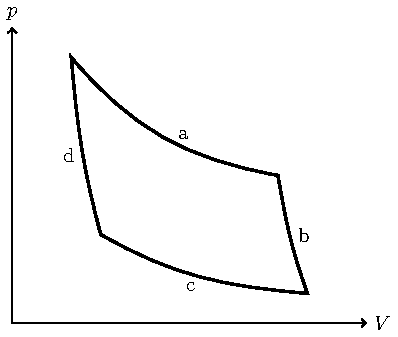
\includegraphics[width = 0.5\textwidth]{./Images/carnot.pdf}
	\caption{Schematic of a Carnot cycle.}
	\label{fig:carnot}
\end{figure}

During step a, the gas expands isothermally, and we have
\begin{align*}
	\Delta U = 0,\ Q = W = nRT_{\text{h}}\ln{\frac{V_{\text{b}}}{V_{\text{a}}}}.
\end{align*}

During step b, the gas expands adiabatically, and we have
\begin{align*}
	Q = 0,\ W = \Delta U = C_{V}(T_{\text{l}} - T_{\text{h}}).
\end{align*}

During step c, the gas compresses isothermally, and we have
\begin{align*}
	\Delta U = 0,\ Q = W = nRT_{\text{l}}\ln{\frac{V_{\text{d}}}{V_{\text{c}}}}.
\end{align*}

During step b, the gas compresses adiabatically, and we have
\begin{align*}
	Q = 0,\ W = \Delta U = C_{V}(T_{\text{h}} - T_{\text{l}}).
\end{align*}

We use the previously derived expressions for adiabatic processes to write
\begin{align*}
	T_{\text{h}}V_{a}^{\gamma - 1} = T_{\text{l}}V_{d}^{\gamma - 1},\ T_{\text{h}}V_{b}^{\gamma - 1} = T_{\text{l}}V_{c}^{\gamma - 1}.
\end{align*}
Thus we obtain for the isothermal compression that
\begin{align*}
	Q = nRT_{\text{l}}\ln(\frac{\left(\frac{T_{\text{h}}}{T_{\text{l}}}\right)^{\frac{1}{\gamma - 1}}V_{a}}{\left(\frac{T_{\text{h}}}{T_{\text{l}}}\right)^{\frac{1}{\gamma - 1}}V_{b}}) = nRT_{\text{l}}\ln(\frac{V_{a}}{V_{b}}),
\end{align*}
and thus $\frac{\abs{Q}}{T}$ is constant for the two heat-exchanging steps.

\paragraph{Efficiency}
The efficiency of a machine has various definitions, but the general definition is the ratio between the energy you get out and the energy you put in.

\paragraph{Carnot's Theorem}
No heat engine working between two heat reservoirs is more efficient than a Carnot engine.

To prove this, suppose that you create an engine producing the same work $W$ as a Carnot heat engine, but for an energy $Q'$ as opposed to the energy $Q$ needed to run the Carnot engine. Now let your new engine be used to power a reversed Carnot engine. As the process must be performed cyclically, the statement that this new engine is more efficient is expressed as
\begin{align*}
	\frac{W}{Q'} > \frac{W}{Q} \implies Q > Q'.
\end{align*}
During the process each engine gives off some heat $Q_{\text{l}}$ to the cold reservoir. The first law of thermodynamics implies
\begin{align*}
	W = Q' - Q_{\text{l}}' = Q - Q_{\text{l}}.
\end{align*}
As $Q - Q' > 0$, so is $Q_{\text{l}} - Q_{\text{l}}'$. Now, $Q - Q'$ is the net energy left in the hot reservoir during a cycle and $Q_{\text{l}} - Q_{\text{l}}'$ is the energy extracted from the cold reservoir. The sole result of this process is thus to extract energy from a cold reservoir to a hot one, which violates the second law.

\subparagraph{Corollary}
All reversible heat engines working between two temperatures have the same efficiency as a Carnot engine.

To show this, suppose a Carnot engine is working between two reservoirs and running another engine undoing that process. This other engine cannot be more efficient than the Carnot engine, meaning that it delivers a greater amount of energy to the hot reservoir than the Carnot engine took, violating the second law of thermodynamics. Thus the two engines must have the same efficiency.

\paragraph{Clausius' Theorem}
Consider some arbitrary cyclic process. We can describe this as a sequence of the system being connected to temperatures $T_{i}$, with heats $\din{Q_{i}}$ being supplied at every stage. The total work performed during the cycle is given by
\begin{align*}
	W = \sum\din{Q_{i}}.
\end{align*}
Now suppose that the heat at each point is supplied by a Carnot engine operating between two reservoirs at temperature $T$ and $T_{i}$. Using the constant ratio for Carnot cycles which was derived previously, we have
\begin{align*}
	\frac{\din{Q_{i}}}{T_{i}} = \frac{\din{Q_{i}} + \din{W_{i}}}{T}
\end{align*}
where $\din{W_{i}}$ is the work done by the Carnot engine. This process cannot violate the second law of thermodynamics, hence
\begin{align*}
	W + \sum\din{W_{i}} \leq 0.
\end{align*}
Hence
\begin{align*}
	\sum\din{Q_{i}} + \sum\din{Q_{i}}\left(\frac{T}{T_{i}} - 1\right) = T\sum\frac{\din{Q_{i}}}{T_{i}} \leq 0.
\end{align*}
The temperature $T$ is constant and positive, and can thus be ignored. In the limit of considering the process in a continuous manner, this becomes
\begin{align*}
	\intin{}{}{Q}{\frac{1}{T}} \leq 0.
\end{align*}
This is Clausius' theorem, where equality necessarily holds for a reversible cycle.

\paragraph{Entropy}
As we have seen, the integral
\begin{align*}
	\intin{}{}{Q}{\frac{1}{T}}
\end{align*}
is path independent for a reversible process. We thus define the state function
\begin{align*}
	\dd{S} = \frac{\din{Q}}{T}
\end{align*}
to be the entropy.

\paragraph{The Second Law and Entropy}
Consider two points connected by a reversible and an irreversible process such that the two form a cycle. Clausius' theorem yields
\begin{align*}
	\intin{A}{B}{Q}{\frac{1}{T}} + \intin{B}{A}{Q_{\text{rev}}}{\frac{1}{T}} \leq 0 \implies \intin{A}{B}{Q}{\frac{1}{T}} \leq \intin{A}{B}{Q_{\text{rev}}}{\frac{1}{T}}.
\end{align*}
This holds for two arbitrary points, meaning
\begin{align*}
	\dd{S} \geq \frac{\din{Q}}{T}.
\end{align*}
Considering a thermally isolated system, we obtain
\begin{align*}
	\dd{S} \geq 0.
\end{align*}
This is a restatement of the second law of thermodynamics, and essentially an equilibrium condition for any isolated system.

\paragraph{The First Law and Entropy}
For a reversible process on a gas we obtain
\begin{align*}
	\dd{U} = T\dd{S} - p\dd{V},
\end{align*}
or more generally
\begin{align*}
	\dd{U} = T\dd{S} + X\dd{x}.
\end{align*}
However, as all involved quantities are functions of state, this must hold even if the process in question is irreversible.

\paragraph{Natural Variables For Internal Energy}
Our restatement of the first law implies that $U$ is most naturally written as a function of $S$ and $x$ (naturally it could be written in terms of other variables too, but you would have to change variables from $S$ and $x$ in order to do that. A switch from $S$ to $T$ would for instance be rewriting $U$ as $U(S(T), x)$). The restatement also implies
\begin{align*}
	\fix{\pdv{U}{S}}{V} = T,\ \fix{\pdv{U}{x}}{S} = X.
\end{align*}

\paragraph{Chemical Potential}
In addition to the dependence of the internal energy on entropy and volume, there is a dependence on the number of particles of type $i$. This is contained in the chemical potential, defined as
\begin{align*}
	\mu_{i} = \fix{\pdv{U}{N_{i}}}{S, x, N_{j}}
\end{align*}
where $j \neq i$. From now on, summation rules will be used for chemical potentials, $i$ will signify all sets of possible values of $i$, and $j\neq i$ may always be assumed to be true unless otherwise specified.

\paragraph{Entropy}
We can re-express the differential of internal energy as a differential of entropy or use the reciprocal and reciprocity theorems to obtain
\begin{align*}
	\dd{S} = \frac{1}{T}\dd{U} - \frac{X}{T}\dd{x}.
\end{align*}
This implies that the entropy is a function of $U$, $x$ and $N_{i}$, as well as
\begin{align*}
	\fix{\pdv{S}{U}}{x, N_{i}} = \frac{1}{T},\ \fix{\pdv{S}{x}}{U, N_{i}} = -\frac{X}{T},\ \fix{\pdv{S}{N_{i}}}{U, x, N_{j}} = -\frac{\mu_{i}}{T}.
\end{align*}

\paragraph{Enthalpy}
%TODO: Continue to rewrite for general systems
The enthalpy is defined as 
\begin{align*}
	H = U + pV.
\end{align*}
We have
\begin{align*}
	\dd{H} = \dd{U} + p\dd{V} + V\dd{p} = T\dd{S} - p\dd{V} + \mu_{i}\dd{N_{i}} + p\dd{V} + V\dd{p} = T\dd{S} + V\dd{p} + \mu_{i}\dd{N_{i}},
\end{align*}
implying that $H$ is a function of $S$, $p$ and $N_{i}$, as well as
\begin{align*}
	\fix{\pdv{H}{S}}{p, N_{i}} = T,\ \fix{\pdv{H}{p}}{S, N_{i}} = V,\ \fix{\pdv{H}{N_{i}}}{S, V,  N_{j}} = \mu_{i}.
\end{align*}

\paragraph{Helmholtz Free Energy}
The Helmholtz free energy is defined as
\begin{align*}
	F = U - TS.
\end{align*}
We have
\begin{align*}
	\dd{F} = \dd{U} - T\dd{S} - S\dd{T} = T\dd{S} - p\dd{V} + \mu_{i}\dd{N_{i}} - T\dd{S} - S\dd{T} = -p\dd{V} - S\dd{T} + \mu_{i}\dd{N_{i}},
\end{align*}
implying that $F$ is a function of $T$, $V$ and $N_{i}$, as well as
\begin{align*}
	\fix{\pdv{F}{T}}{V, N_{i}} = -S,\ \fix{\pdv{F}{V}}{T, N_{i}} = -p,\ \fix{\pdv{F}{N_{i}}}{T, V,  N_{j}} = \mu_{i}.
\end{align*}

\paragraph{Gibbs Free Energy}
The Gibbs free energy is defined as
\begin{align*}
	G = H - TS.
\end{align*}
We have
\begin{align*}
	\dd{G} = \dd{H} - T\dd{S} - S\dd{T} = T\dd{S} + V\dd{p} + \mu_{i}\dd{N_{i}} - T\dd{S} - S\dd{T} = V\dd{p} - S\dd{T} + \mu_{i}\dd{N_{i}},
\end{align*}
implying that $G$ is a function of $T$, $p$ and $N_{i}$, as well as
\begin{align*}
	\fix{\pdv{G}{T}}{p} = -S,\ \fix{\pdv{G}{p}}{T} = V,\ \fix{\pdv{G}{N_{i}}}{T, p,  N_{j}} = \mu_{i}.
\end{align*}

\paragraph{The Grand Potential}
The grand potential is defined as
\begin{align*}
	\GP = F - \mu_{i}N_{i}.
\end{align*}
We have
\begin{align*}
	\dd{\GP} = -p\dd{V} - S\dd{T} + \mu_{i}\dd{N_{i}} - \mu_{i}\dd{N_{i}} - N_{i}\dd{\mu_{i}} = -p\dd{V} - S\dd{T} - N_{i}\dd{\mu_{i}},
\end{align*}
implying that $\GP$ is a function of $V$, $T$ and $\mu_{i}$, as well as
\begin{align*}
	S = - \fix{\pdv{\GP}{T}}{V, \mu},\ p = - \fix{\pdv{\GP}{V}}{T, \mu},\ N_{i} = - \fix{\pdv{\GP}{\mu_{i}}}{T, V, N_{j}}.
\end{align*}

\paragraph{Availability and Equilibrium}
The availability is a more general quantity which can be defined appropriately for systems with given constraints. Its differential will give both the maximal amount of work that can be performed by a system and a general equilibrium condition for the system.

As an example, consider a system in contact with surroundings at temperature $T_{0}$ and pressure $p_{0}$ (which may be chosen independently of the constraints on the system as both pressure and temperature are extensive and we assume the surroundings to be much larger than the system). If heat $\din{Q}$ is supplied to the system during some process, the entropy change satisfies $T_{0}\dd{S} \geq \din{Q}$, where $S$ is the entropy of the system. The first law implies
\begin{align*}
	\din{Q} = \dd{U} - \din{W} - (-p_{0}\dd{V}),
\end{align*}
where we have separated the work into a term arising due to the change in volume and a term describing other sources. Combining this yields
\begin{align*}
	T_{0}\dd{S} &\geq \dd{U} - \din{W} - (-p_{0}\dd{V}), \\
	\din{W}     &\geq \dd{U} - T_{0}\dd{S}  + p_{0}\dd{V}.
\end{align*}
Defining the availability for this case as
\begin{align*}
	A = U + p_{0}V - T_{0}S
\end{align*}
implies
\begin{align*}
	\din{W} \geq \dd{A},
\end{align*}
where equality is obtained for a reversible processes. Thus changes in the availability are equal to the maximal amount of useful work that can be extracted from a system.

If the system is mechanically isolated from the surroundings, such that only volume-changing work can be performed, we have
\begin{align*}
	\dd{A} \leq 0.
\end{align*}
Looking more closely at the differential of the availability, we obtain
\begin{align*}
	\dd{A} = \dd{U} + p_{0}\dd{V} - T_{0}\dd{S} = \dd(U + p_{0}V - T_{0}S) = \dd{G}.
\end{align*}
Hence the equilibrium condition is that Gibbs free energy is minimized.

In a similar fashion we find that for thermally isolated systems at fixed volume, the appropriate availability is $A = -T_{0}S$, and hence for such systems the entropy is maximized. For a system at fixed temperature and volume the appropriate availability is $A = U - T_{0}S = F$, and hence for such systems the Helmholtz free energy is minimized.

\paragraph{Exchanges Between Systems}
For systems in contact, equilibrium is determined by minimizing the total availability.

As an example, consider two systems at fixed volume in thermal contact. For such a system the equilibrium condition is that the entropy is maximized. We obtain
\begin{align*}
	\dd{S} = \dd{S_{1}} + \dd{S_{2}} = \frac{1}{T_{1}}\dd{U_{1}} + \frac{1}{T_{2}}\dd{U_{2}} \geq 0.
\end{align*}
Energy conservation implies that the two internal energy changes must balance each other, yielding
\begin{align*}
	\left(\frac{1}{T_{1}} - \frac{1}{T_{2}}\right)\dd{U_{1}} \geq 0,
\end{align*}
and hence the systems reach equilibrium when they reach the same temperature.

\paragraph{Maxwell Relations}
Using the symmetry of partial derivatives for a state function, one can obtain relations between derivatives of other state functions.

As an example, the derivatives of $F$ are $-S$ and $-p$, computed with respect to $T$ and $V$. This implies
\begin{align*}
	\fix{\pdv{S}{V}}{T} = \fix{\pdv{p}{T}}{V}.
\end{align*}

\paragraph{The Third Law}
The third law was initially concerned with the issue of determining absolute entropies. Three different statements of the third law were finally coined:

\begin{itemize}
	\item \textbf{Nernst's statement:} Near absolute zero, all reactions in a system in internal equilibrium take place with no change in entropy.
	\item \textbf{Planck's statement:} The entropy of all systems in internal equilibrium is the same at absolute zero, and may be taken to be zero.
	\item \textbf{Simon's satement:} The contribution to the entropy of a system by each aspect of the system which is in internal thermodynamic equilibrium tends to zero when approaching absolute zero.
\end{itemize}

Simon's idea of aspects are based on a closer and closer inspections of a system. Considering a crystal for instance, it can be studied as a macroscopic entity or in terms of the individual atoms comprising it. These are, in turn, built up of nucleons, which are made up of quarks and so on (potentially). Each of these is termed an aspect.

\paragraph{Consequences of the Third Law}
Now we examine some of the consequences of the third law.

The first consequence is for heat capacities. We have
\begin{align*}
	C = T\pdv{S}{T} = \pdv{S}{\ln{T}} \to 0.
\end{align*}
One might suspect that the first equality implies it (and I don't know why it does not). But the second statement guarantees it, as the third law implies that the entropy is bounded at low temperatures.

A second consequence is for thermal expansion. The third law implies
\begin{align*}
	\fix{\pdv{S}{p}}{T} \to 0
\end{align*}
near absolute zero, which implies
\begin{align*}
	\fix{\pdv{V}{T}}{p} \to 0.
\end{align*}

A third consequence is for ideal systems, such as the ideal gas and non-interacting spin systems. These cannot be ideal at low temperatures, a fact that might be guessed at based on tendencies in their entropies, but can also be justified by the fact that interactions between units in the system can be disregarded at high temperatures, where the ideal models are valid, but not at lower temperatures.

A final consequence is the fact that one cannot cool to $T = 0$ in a finite number of steps, a fact which is not easy to prove rigorously.

\paragraph{Reinterpretation of the Chemical Potential and Grand Potential}
Consider a system of only one kind of particles which is scaled by a factor $\lambda$. The entropy, expressed as a function of $U$, $V$ and $N$ is extensive, yielding that it, too, is scaled by a factor $\lambda$. Let a subscript $\lambda$ denote quantities for a scaled system. We thus have
\begin{align*}
	S_{\lambda} = \lambda S.
\end{align*}
Differentiating with respect to $\lambda$ 
\begin{align*}
	S &= \fix{\pdv{S_{\lambda}}{U_{\lambda}}}{V_{\lambda}, N_{\lambda}}\pdv{U_{\lambda}}{\lambda} + \fix{\pdv{S_{\lambda}}{V_{\lambda}}}{U_{\lambda}, N_{\lambda}}\pdv{V_{\lambda}}{\lambda} + \fix{\pdv{S_{\lambda}}{N_{\lambda}}}{U_{\lambda}, V_{\lambda}}\pdv{N_{\lambda}}{\lambda}.
\end{align*}
Setting $\lambda = 1$ or arguing that temperature is intensive yields that this is equal to
\begin{align*}
	S = \frac{U}{T} + \frac{p}{T} - \frac{\mu}{T}. 
\end{align*}
We can rewrite this as
\begin{align*}
	U - TS + pV = G = \mu N,
\end{align*}
and thus that $\mu$ is the Gibbs free energy per particle. This also implies
\begin{align*}
	\GP = -pV.
\end{align*}

%TODO: Show for multiple kinds of particles

\paragraph{Chemical Potential Without Particle Conservation}
For certain systems, there are no conservation laws for the number of particles. In such cases, if the chemical potential is fixed, the system will evolve in such a way as to minimize the availability with respect to the number of particles, which corresponds to $\mu = 0$. If there is a conservation law present, one must instead construct a constraint on the chemical potentials.

\paragraph{Gaseous Chemical Reactions}

\paragraph{Latent Heat}
Consider a phase transition. During such a transition the temperature is constant, and in order for the transition to occur a certain amount of heat must be supplied. This is called the latent heat and is given by
\begin{align*}
	L = T_{\text{c}}\Delta S.
\end{align*}

\paragraph{Trouton's Rule}
For an interaction-free fluid, the multiplicity is proportional to the volume, yielding that the molar multiplicity ratio is
\begin{align*}
	\frac{\Omega_{\text{vapour}}}{\Omega_{\text{liquid}}} = \left(\frac{V_{\text{vapour}}}{V_{\text{liquid}}}\right)^{N_{A}} = \left(\frac{\rho_{\text{liquid}}}{\rho_{\text{vapour}}}\right)^{N_{A}} \approx 10^{3N_{A}},
\end{align*}
as liquids are approximately $1000$ times as dense as vapours. The molar latent heat of fusion is thus
\begin{align*}
	\frac{L}{n} = 7RT_{\text{c}}.
\end{align*}

\paragraph{The Clausius-Clapeyron Equation}
Consider two phases, denoted $1$ and $2$, in equilibrium. We are interested in computing the coexistence curve between the two phases, i.e. the curve of all points such that the two phases are in equilibrium.

At any point of coexistence we have
\begin{align*}
	\dd{G} = \mu_{1}\dd{N_{1}} + \mu_{2}\dd{N_{2}} = 0.
\end{align*}
Conservation of particle number implies that
\begin{align*}
	\mu_{1} = \mu_{2}.
\end{align*}
Now, supposing we were to move along the coexistence curve in the $p-T$ plane, we would have
\begin{align*}
	-s_{1}\dd{T} + v_{1}\dd{p} = -s_{2}\dd{T} + v_{2}\dd{p}
\end{align*}
where $s$ and $v$ are entropies and volumes per particle. This implies
\begin{align*}
	\dv{p}{T} = \frac{s_{2} - s_{1}}{v_{2} - v_{1}} = \frac{l}{T(v_{2} - v_{1})},
\end{align*}
where $l$ is the latent heat per particle. We finally obtain
\begin{align*}
	\dv{p}{T} = \frac{L}{T(V_{2} - V_{1})},
\end{align*}
which is the Clausius-Clapeyron equation.

\end{document}
